% VUT FIT MITAI
% MSZ 2021/2022
% Author: Vladimir Dusek
% Login: xdusek27

%%%%%%%%%%%%%%%%%%%%%%%%%%%%%%%%%%%%%%%%%%%%%%%%%%%%%%%%%%%%%%%%%%%%%%%%%%%%%%%%

% Path to figures
\graphicspath{{wap/bezpecnost_webovych_aplikaci/figures}}

%%%%%%%%%%%%%%%%%%%%%%%%%%%%%%%%%%%%%%%%%%%%%%%%%%%%%%%%%%%%%%%%%%%%%%%%%%%%%%%%

\chapter{WAP~--~Bezpečnost webových aplikací (SOP, XSS, CSRF, bezpečnostní hlavičky HTTP).}

%%%%%%%%%%%%%%%%%%%%%%%%%%%%%%%%%%%%%%%%%%%%%%%%%%%%%%%%%%%%%%%%%%%%%%%%%%%%%%%%

\section{Zdroje}

\begin{compactitem}
    \item \path{WAP10_Bezpecnost.pdf}
    \item \path{WAP_2021-04-15.mp4}
\end{compactitem}

%%%%%%%%%%%%%%%%%%%%%%%%%%%%%%%%%%%%%%%%%%%%%%%%%%%%%%%%%%%%%%%%%%%%%%%%%%%%%%%%

\section{Úvod a kontext}

\begin{compactitem}
    \item Pouhé načtení webové stránky znamená vykonání cizího (Javascript) kódu v počítači.

    \item Výrobci prohlížečů vyvažují dva cíle: \begin{compactitem}
        \item Tvorba API umožňujících přístup k HW a SW uživatelského počítače (grafická karta, geolokace, mikrofon, kamera, \ldots).

        \item Zamezení/omezení dopadů škodlivého kódu (ochrana soukromí, úprava dat, podvody, \ldots).
    \end{compactitem}
\end{compactitem}

%%%%%%%%%%%%%%%%%%%%%%%%%%%%%%%%%%%%%%%%%%%%%%%%%%%%%%%%%%%%%%%%%%%%%%%%%%%%%%%%

\section{Správa sezení}

\begin{compactitem}
    \item Vzhledem k tomu, že protokol HTTP je bezstavový, potřebujeme způsob jak asociovat jeden HTTP request druhému, tedy způsob jak ukládat uživatelská data mezi HTTP requesty.

    \item Soubory cookie nebo parametry URL (např. jako \url{example.com?asd=lol&boo=no}) jsou vhodnými způsoby přenosu dat mezi dvěma nebo více požadavky. Nejsou však vhodné v případě, že nechceme, aby tato data byla čitelná/editovatelná na straně klienta. \begin{compactitem}
        \item Cookies jsou malé bloky dat vytvořené webovým serverem během prohlížení webových stránek uživatelem a uložené do jeho počítače nebo jiného zařízení jeho webovým prohlížečem.
    \end{compactitem}

    \item Řešením je uložit tato data na straně serveru, dát jim id a nechat klienta znát (a předat zpět při každém http požadavku) pouze toto id. ID je na straně klienta uloženo jako cookie.

    \item Sezení (session) je tedy ustanovené síťové spojení mezi klientem a serverem.

    \item Možné útoky: \begin{compactitem}
        \item Krádež sezení -- získání hodnoty ID sezení útočníkem.
        \item Vnucení sezení -- vložení útočníkova ID sezení k oběti.
    \end{compactitem}

    \item Jak zabránit odcizení ID sezení? \begin{compactitem}
        \item Cookies jsou přenášeny pouze přes HTTPS.
        \item Cookies není dostupné přes Javascript, je dostupné pouze přes HTTP.
        \item Nastavení délky sezení (automatické odhlášení).
        \item Změna ID sezení, pokud se provede nějaká akce (přihlášení/odhlášení, citlivá akce -- změna hesla, úprava oprávnění, \ldots).
    \end{compactitem}

\end{compactitem}

%%%%%%%%%%%%%%%%%%%%%%%%%%%%%%%%%%%%%%%%%%%%%%%%%%%%%%%%%%%%%%%%%%%%%%%%%%%%%%%%

\section{Same-origin policy (SOP)}

\begin{compactitem}
    \item Origin (původ), definovaný trojicí URI segemntů ---- schéma, doména, port.

    \item SOP je důležitý bezpečnostní mechanismus, který omezuje způsob, jakým může dokument nebo skript načtený jedním origin interagovat se zdrojem z jiného origin. \begin{compactitem}
        \item Webový prohlížeč povolí skriptům obsaženým na první webové stránce přístup k datům na druhé webové stránce, ale pouze v případě, že obě webové stránky mají stejný origin.
    \end{compactitem}

    \item SOP zabraňuje tomu, aby škodlivý skript na jedné stránce získal přístup k citlivým datům na jiné webové stránce prostřednictvím jejího DOM.

    \item Příklad: \begin{compactitem}
        \item Webová aplikace je dostupná na url \url{https://jakjsmenatom.cz}.
        \item Její API je dostupné na url \url{https://api.jakjsmenatom.cz}.
        \item Při SOP, API komunikuje pouze se subdoménami \url{jakjsmenatom.cz}, z jiné domény nelze API dotazovat.
    \end{compactitem}

    \item Útok: \textbf{Postraní kanály obcházející SOP} \begin{compactitem}
        \item SOP brání přečtení odpovědi $\rightarrow$ nebrání však odeslání požadavku. \begin{compactitem}
            \item XHR na origin mimo SOP.
            \item Obrázek s atributem src mimo SOP.
        \end{compactitem}
        \item XHR generuje událost load při existenci zdroje, i když prohlížeč přístup k obsahu odmítne. \begin{compactitem}
            \item Podle událostí error, či timeout lze zjistit otevřené porty.
        \end{compactitem}
        \item V kombinaci s CSRF lze měnit stav na serveru.
    \end{compactitem}
\end{compactitem}

%%%%%%%%%%%%%%%%%%%%%%%%%%%%%%%%%%%%%%%%%%%%%%%%%%%%%%%%%%%%%%%%%%%%%%%%%%%%%%%%

\section{Cross-site scripting (XSS)}

\begin{compactitem}
    \item Útočník vloží značky nebo skripty do cílové stránky. \begin{compactitem}
        \item Kód se vykoná, když uživatel navštíví stránku.
    \end{compactitem}

    \item Stránka je zranitelná pokud: \begin{compactitem}
        \item Zobrazuje obsah na základě uživatelských vstupů, které jsou bez dostatečné validace.
    \end{compactitem}

    \begin{figure}[H]
        \centering
        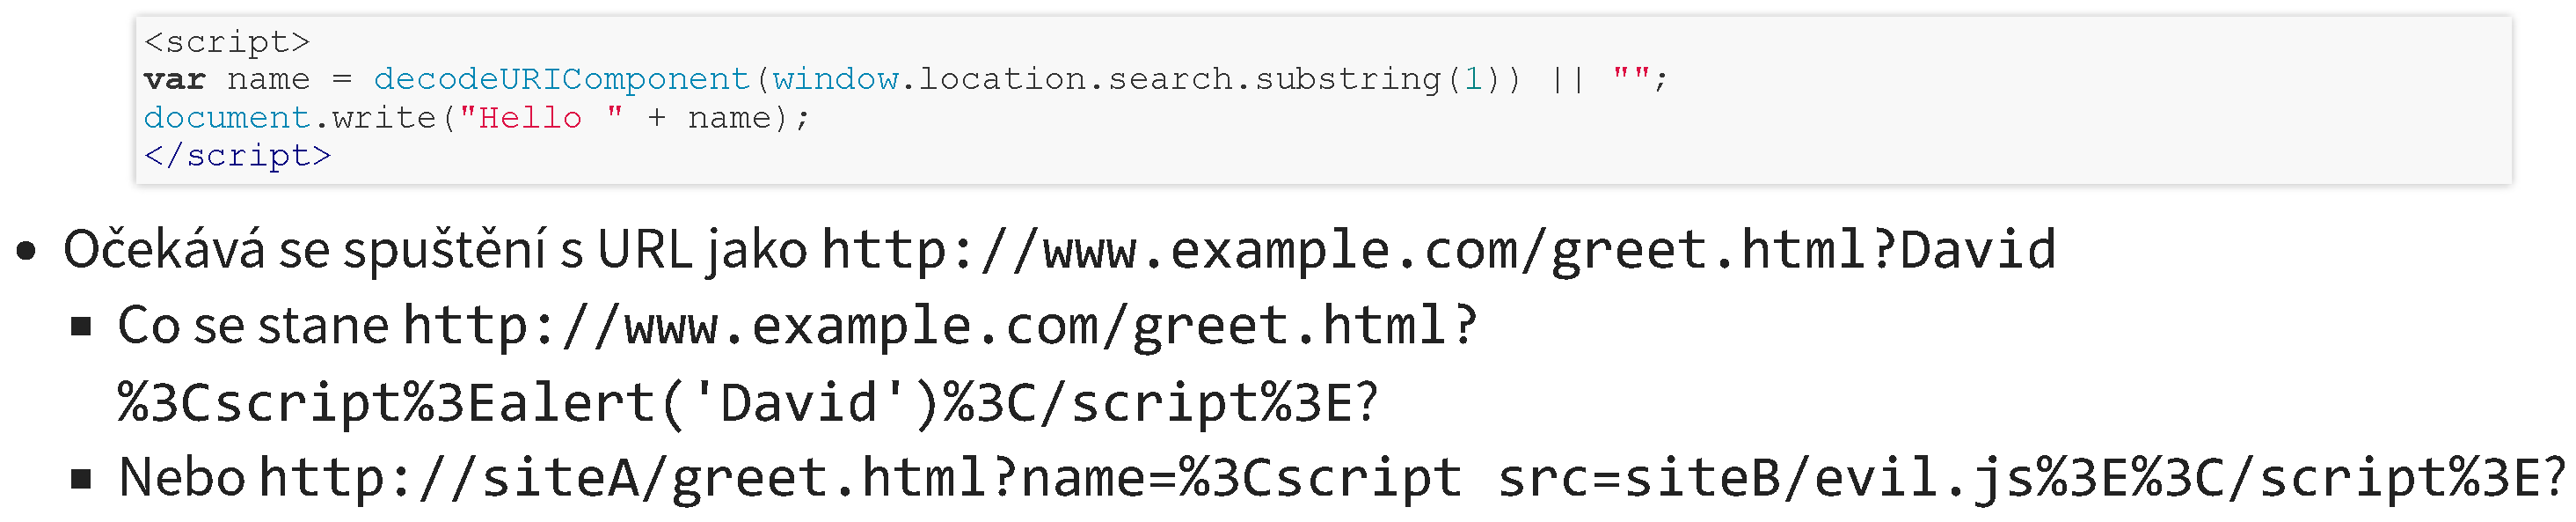
\includegraphics[width=1\linewidth]{xss_priklad.pdf}
        \caption{Příklad XSS.}
    \end{figure}

    \item Varianty XSS: \begin{compactitem}
        \item Trvalé (perzistentní), uložené v databázi.
        \item Dočasné.
        \item Lokální (DOM based)
    \end{compactitem}

    \item Jak realizovat? \begin{compactitem}
        \item Zkracovače odkazů, přesměrování (hlavička Location), znaky kódované pomocí reprezentace ASCII, \ldots
    \end{compactitem}

    \item Nebezpečí XSS: odcizení cookies, obsah web storage, zmáčknuté klávesy, pohyb myši, upravovat formuláře, těžba kryptoměn.

    \item Řešení: \begin{compactitem}
        \item sanitizace vstupů;

        \item HTTP hlavička \textbf{Content Security Policy}: \begin{compactitem}
            \item Zakázání prohlížeči stahování zdrojů mimo povolené origin.
            \item CSP poskytuje majitelům webových stránek standardní metodu pro deklarování schváleného původu obsahu, který by měly prohlížeče na dané webové stránce povolit načítat.
        \end{compactitem}

        \item HTTP hlavička \textbf{Feature policy}: \begin{compactitem}
            \item Stránka vyžaduje, nebo nevyžaduje určité vlastnosti (např. zobrazení na fullscreen, přístup k poloze \ldots).
            \item Omezení přístupu Javascriptu k browser API (např. zakázání přístupu k poloze).
        \end{compactitem}
    \end{compactitem}
\end{compactitem}

%%%%%%%%%%%%%%%%%%%%%%%%%%%%%%%%%%%%%%%%%%%%%%%%%%%%%%%%%%%%%%%%%%%%%%%%%%%%%%%%

\section{Cross-site request forgery (CSRF)}

\begin{compactitem}
    \item Útočník přinutí uživatele změnit stav ve webové aplikaci, ke které je již přihlášený.
    \item Změna stavu, ne krádež dat. -- Útočník nemá přístup k odpovědi na změnu stavu.
    \item Není porušená důvěrnost, ale je porušena integrita.

    \begin{figure}[H]
        \centering
        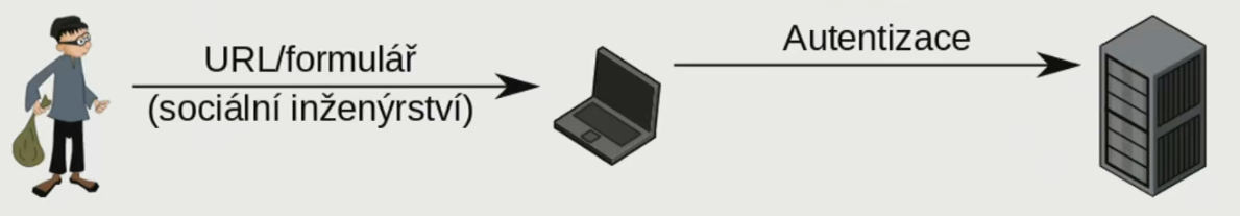
\includegraphics[width=1\linewidth]{csrf_1.pdf}
        \caption{Princip CSRF, část 1.}
    \end{figure}

    \begin{figure}[H]
        \centering
        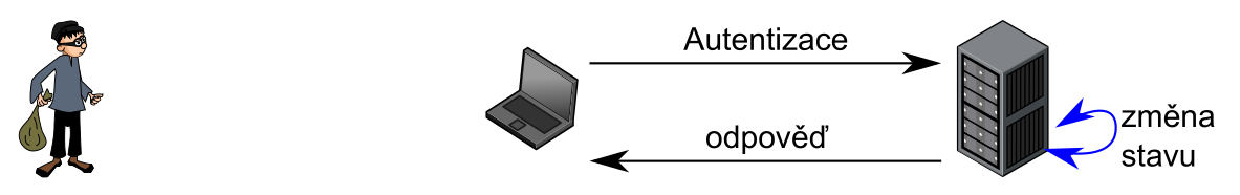
\includegraphics[width=1\linewidth]{csrf_2.pdf}
        \caption{Princip CSRF, část 2.}
    \end{figure}

    \begin{figure}[H]
        \centering
        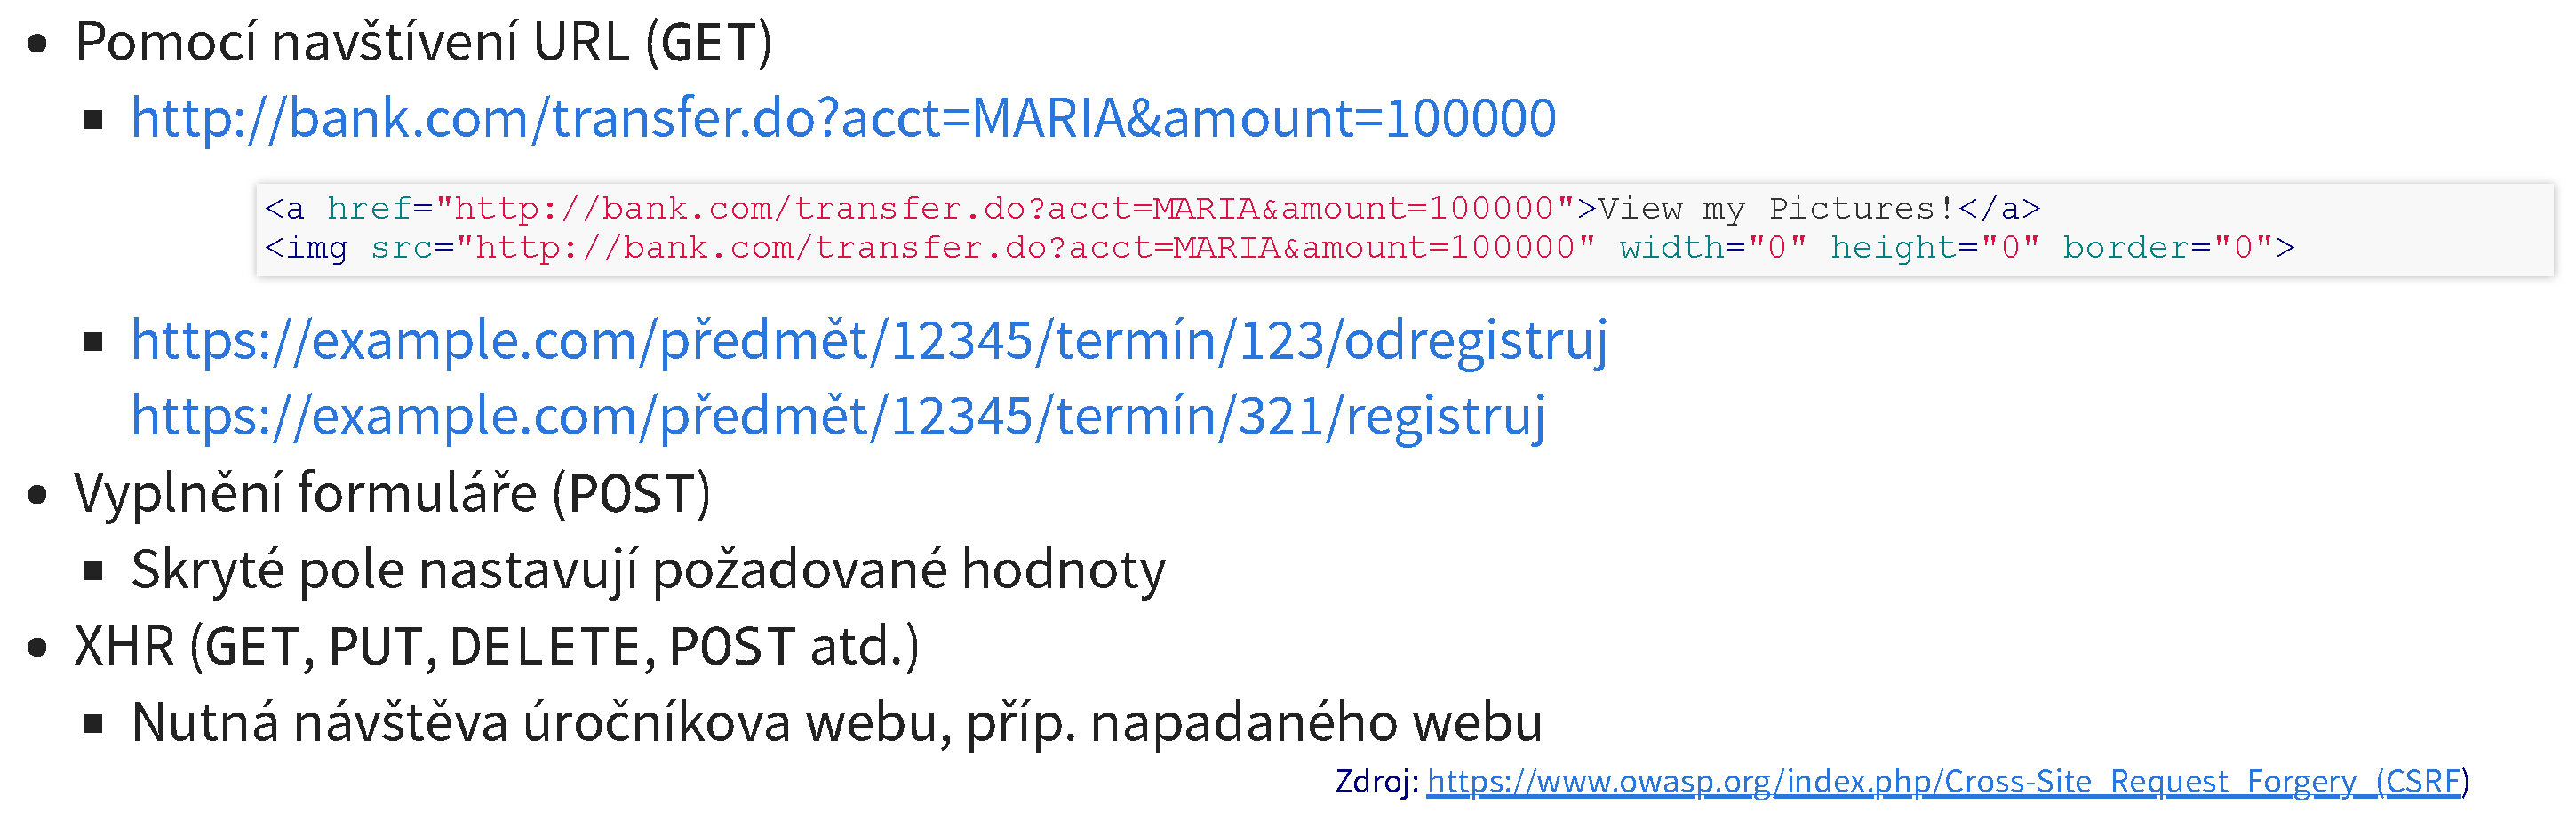
\includegraphics[width=1\linewidth]{csrf_realizace.pdf}
        \caption{Jak je možné realizovat CSRF útok.}
    \end{figure}

    \item Obrana proti CSRF -- \textbf{Synchronizační token} \begin{compactitem}
        \item Každá zmena stavu závisí na náhodném unikátním tokenu (unikátní pro sezení).
        \item Token je unikátní pro konkrétní operací, obsahuje zašifrované informace klíčem dostupným jen serveru -- typ operace, čas operace, jméno uživatele, nonce, unikátní náhodný řetězec.
        \item Token použit \begin{compactitem}
            \item Součástí URL GET měnících stav -- Lépe: nepoužívat GET definovaný jako bezpečná metoda pro změnu stavu.
            \item Součástí požadavků PUT, DELETE aj. prováděných pomocí XHR.
            \item Skryté pole ve formulářích.
        \end{compactitem}
    \end{compactitem}

    \item Obrana proti CSRF -- \textbf{HTTP hlavičky} \begin{compactitem}
        \item Kontrola hlavičky Origin \begin{compactitem}
            \item Origin: \url{https://fit.vutbr.cz}
            \item Obsahuje origin, ze kterého pochází dotaz.
            \item Kontrola, zda odpovídá očekávanému (pokud je součásti dotazu).
        \end{compactitem}

        \item Kontrola hlavičky Referer \begin{compactitem}
            \item Referer: \url{https://fit.vutbr.cz/study/courses/WAP/private/lectures/2019.php?p=bezpečn}
            \item URL naposledy zobrazené stránky.
            \item Kontrola, zda odpovídá očekávanému (pokud je součásti dotazu).
        \end{compactitem}
    \end{compactitem}

    \item Obrana proti CSRF -- \textbf{Interakce uživatele} \begin{compactitem}
        \item Nová autentizace.
        \item Jednorázově použitelný token (explictně zadaný uživatelem).
        \item CAPTCHA.
    \end{compactitem}
\end{compactitem}

%%%%%%%%%%%%%%%%%%%%%%%%%%%%%%%%%%%%%%%%%%%%%%%%%%%%%%%%%%%%%%%%%%%%%%%%%%%%%%%%

\section{Bezpečnostní hlavičky HTTP}

\begin{compactitem}
    \item Pomocí bezpečnostních HTTP hlaviček můžeme nastavit různá pravidla pro komunikaci mezi webovým prohlížečem a serverem.

    \item Typicky umožňují povolit nebo zakázat určité funkce prohlížeče pro vyšší bezpečnost a soukromí.

    \item Např. Content Security Policy, Feature Policy, Strict-Transport-Security, X-Frame-Options.
\end{compactitem}

\subsection{HTTPS stripping}

\begin{compactitem}
    \item Man in the middle útok.
    \item Postup: \begin{compactenum}
        \item Uživatel vynechá schéma URI, např. www.example.com.
        \item Výchozí schéma je http.
        \item Útočník nepropaguje přesměrování na HTTPS.
    \end{compactenum}

    \begin{figure}[H]
        \centering
        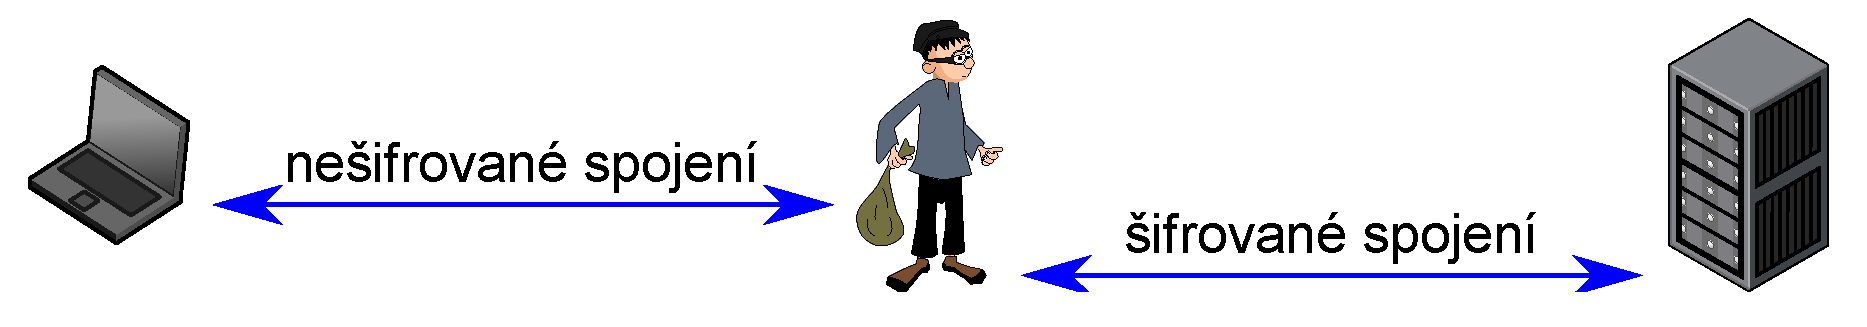
\includegraphics[width=0.9\linewidth]{https_stripping.pdf}
        \caption{Útočník MITM přiměje oběť k přístupu přes HTTP.}
    \end{figure}

    \item HTTP hlavička \textbf{HTTP Strict-Transport-Security} \begin{compactitem}
        \item Na této doméně se vždy šifruje (platí pro všechny porty).
        \item Při HTTP server pošle výzvu, že jakékoliv HTTP požadavky předělat na HTTPS.
    \end{compactitem}
\end{compactitem}

\subsection{Clickjacking}

\begin{compactitem}
    \item Zobrazení několika vrstev prvků přes sebe (neviditelná vrstva).
    \item Uživatel si myslí, že kliká na něco jiného než ve skutečnosti.
    \item Při útoku jsou využívány plovoucí rámce (iframe).
    \item Řešení spočívá v zakázání/omezení zobrazení stránky v iframe.

    \item HTTP hlavička \textbf{X-Frame-Options} \begin{compactitem}
        \item Povoluje/zakazuje/omezuje zobrazení stránky v rámci iframe.
    \end{compactitem}

    \item Hlavička \textbf{Content Security Policy}.
\end{compactitem}
